\chapter{Построение низкоразмерных моделей при вариациях положения управляющих воздействий}\label{ch:ch3}

\todo{4 pages}

\begin{equation}
    \deriv{u}{t} - \varkappa \deriv[2]{u}{x} = q
\end{equation}

\begin{figure}[ht]
    \centerfloat{
        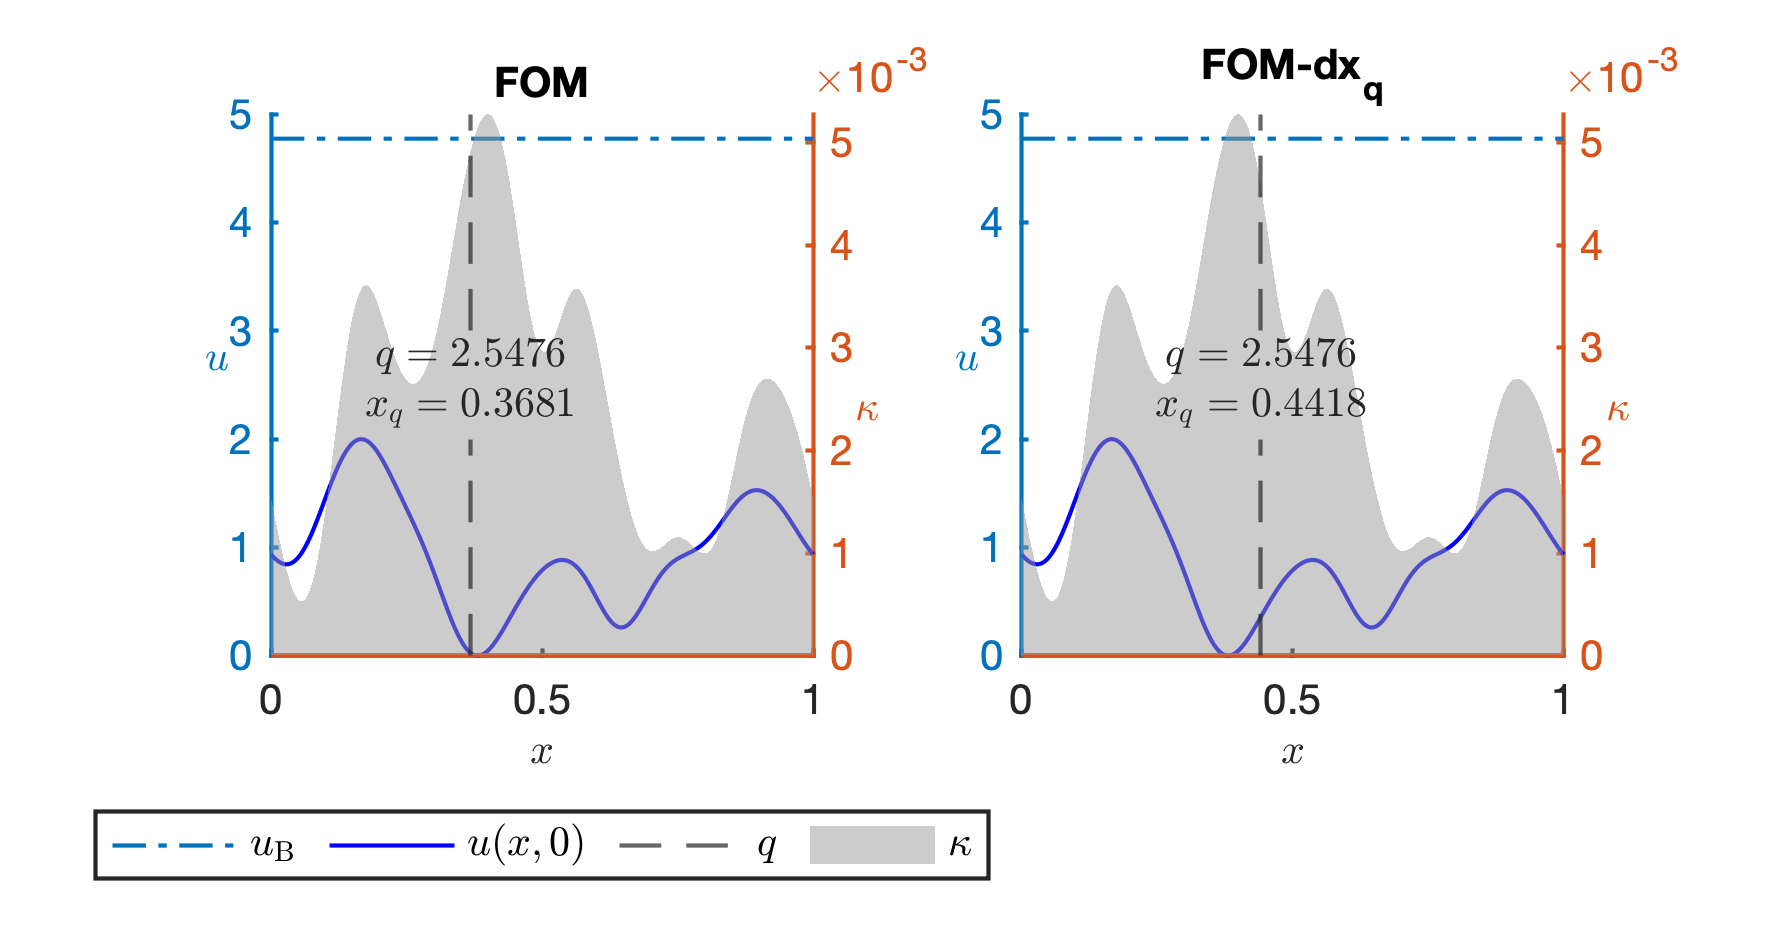
\includegraphics[scale=1]{sci_report/images/ECMOR/8-FOM-Q.png}
    }
    \caption{\todo{caption}~\cite{Elizarev2022}}\label{fig:q-deviation}
\end{figure}

\begin{figure}[ht]
    \centerfloat{
        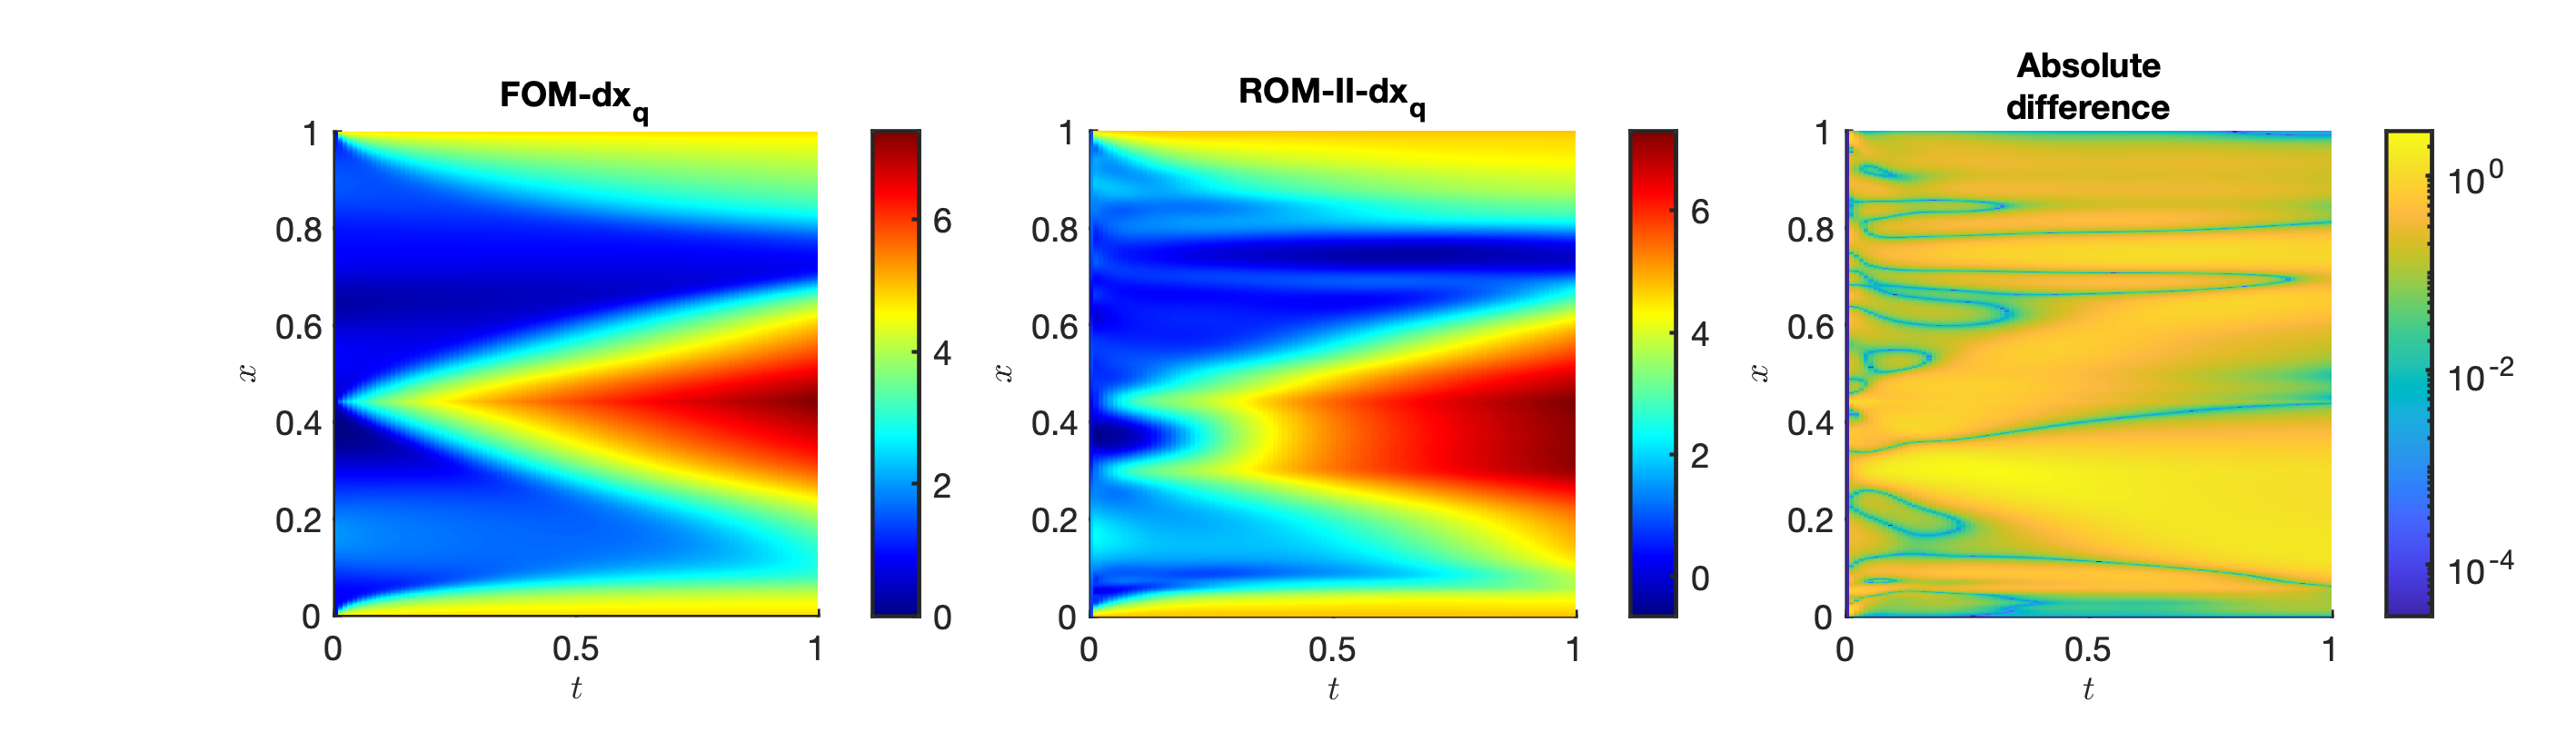
\includegraphics[width=\textwidth]{sci_report/images/ECMOR/9-Problem-Q.png}
    }
    \caption{\todo{caption}~\cite{Elizarev2022}}\label{fig:q-diff}
\end{figure}

\begin{align}
    \deriv{\check{t}}{t} = \alpha = \text{const} \\
    \deriv{\check{x}}{x} = \beta = \text{const} \\
\end{align}

\begin{equation}
    \deriv{u}{\check{t}} - \frac{\beta^2}{\alpha} \varkappa \deriv[2]{u}{\check{x}} = \frac{q}{\alpha}
\end{equation}


\begin{figure}[ht]
    \centerfloat{
        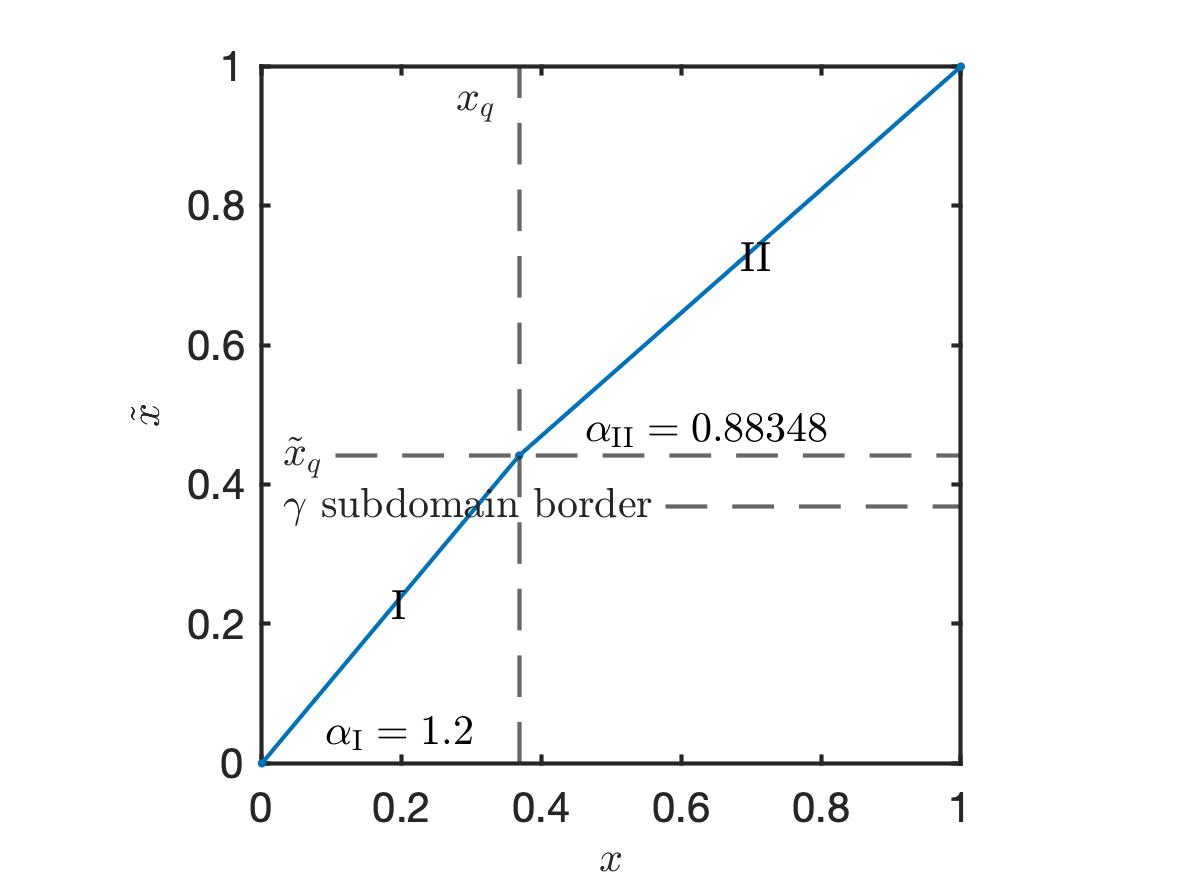
\includegraphics[scale=1.2]{sci_report/images/ECMOR/12-Domains.png}
    }
    \caption{\todo{caption}~\cite{Elizarev2022}}\label{fig:domains}
\end{figure}

\begin{figure}[ht]
    \centerfloat{
        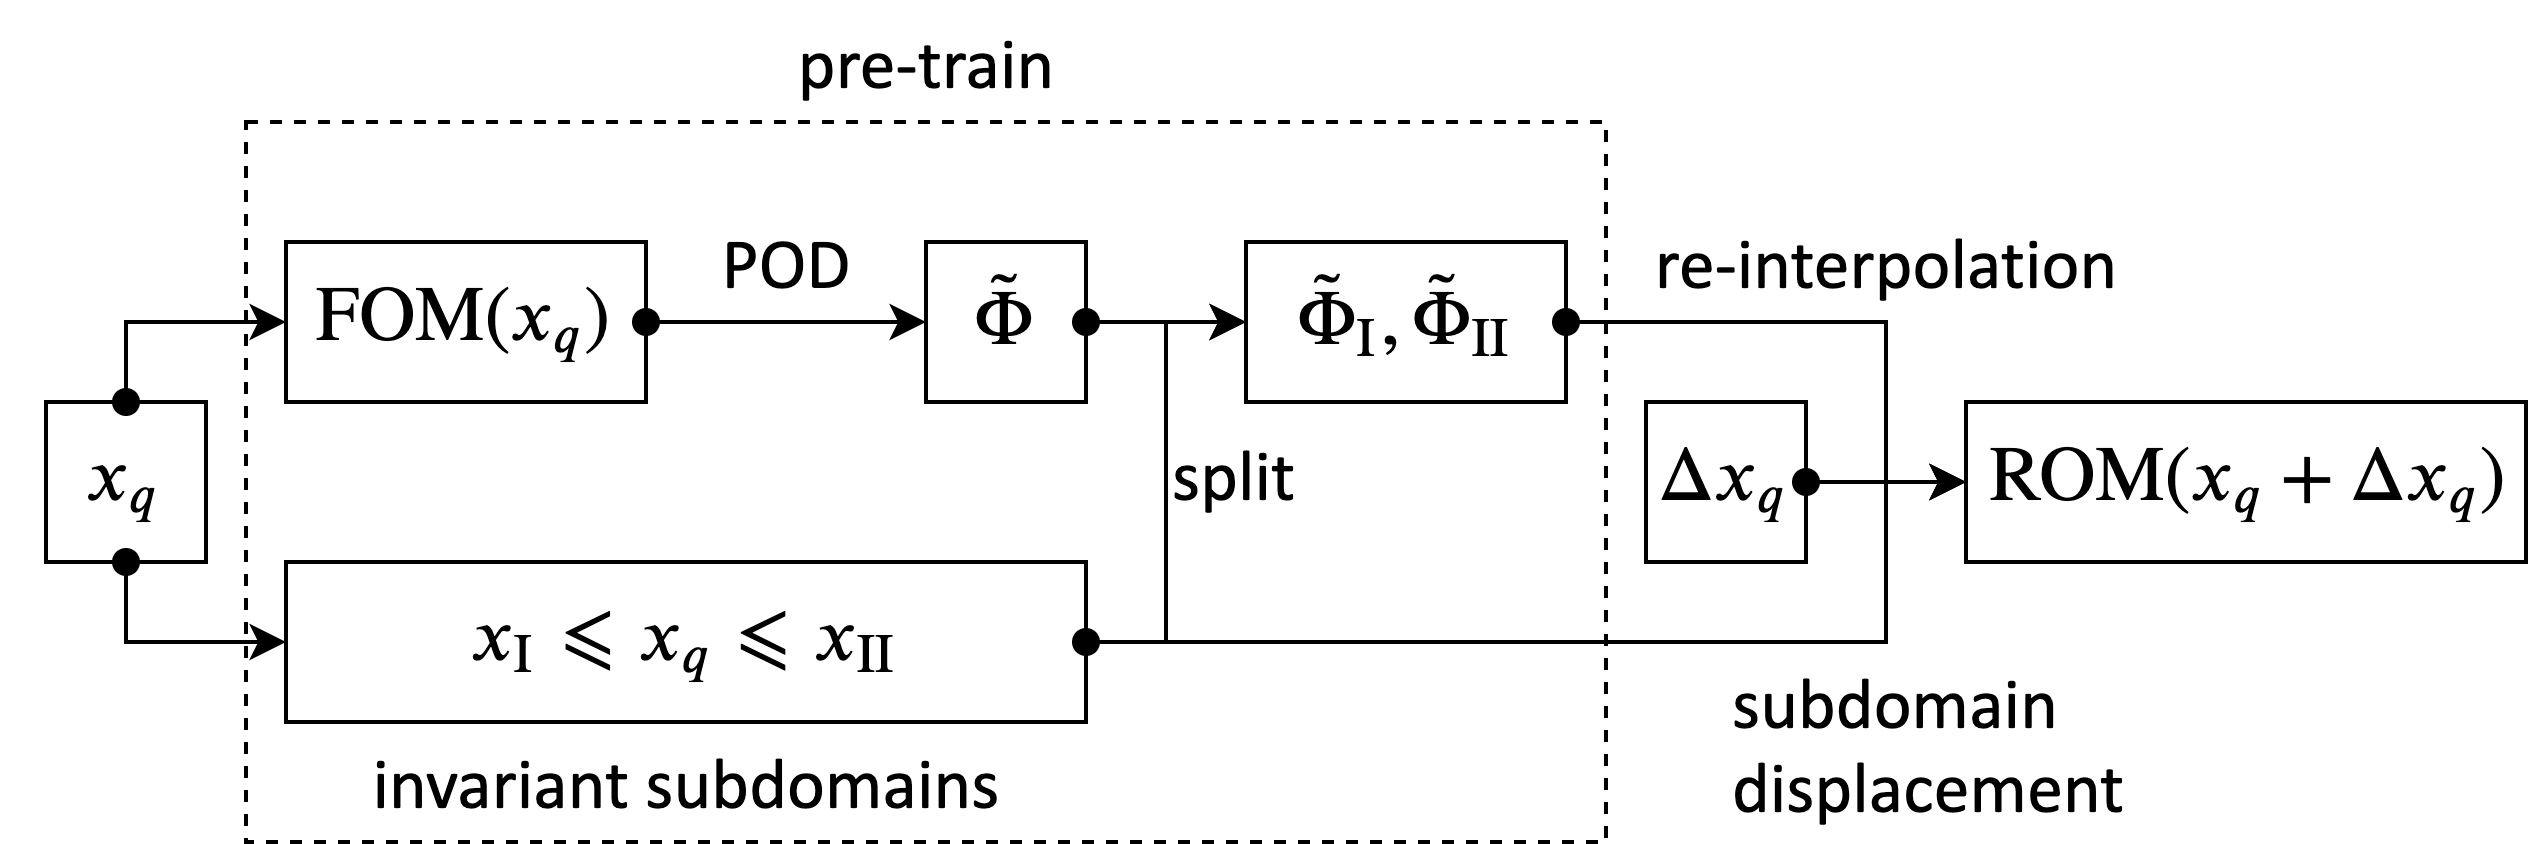
\includegraphics[width=\textwidth]{sci_report/images/ECMOR/DWC-POD.png}
    }
    \caption{\todo{caption}~\cite{Elizarev2022}}\label{fig:dw-scheme}
\end{figure}

\begin{figure}[ht]
    \centerfloat{
        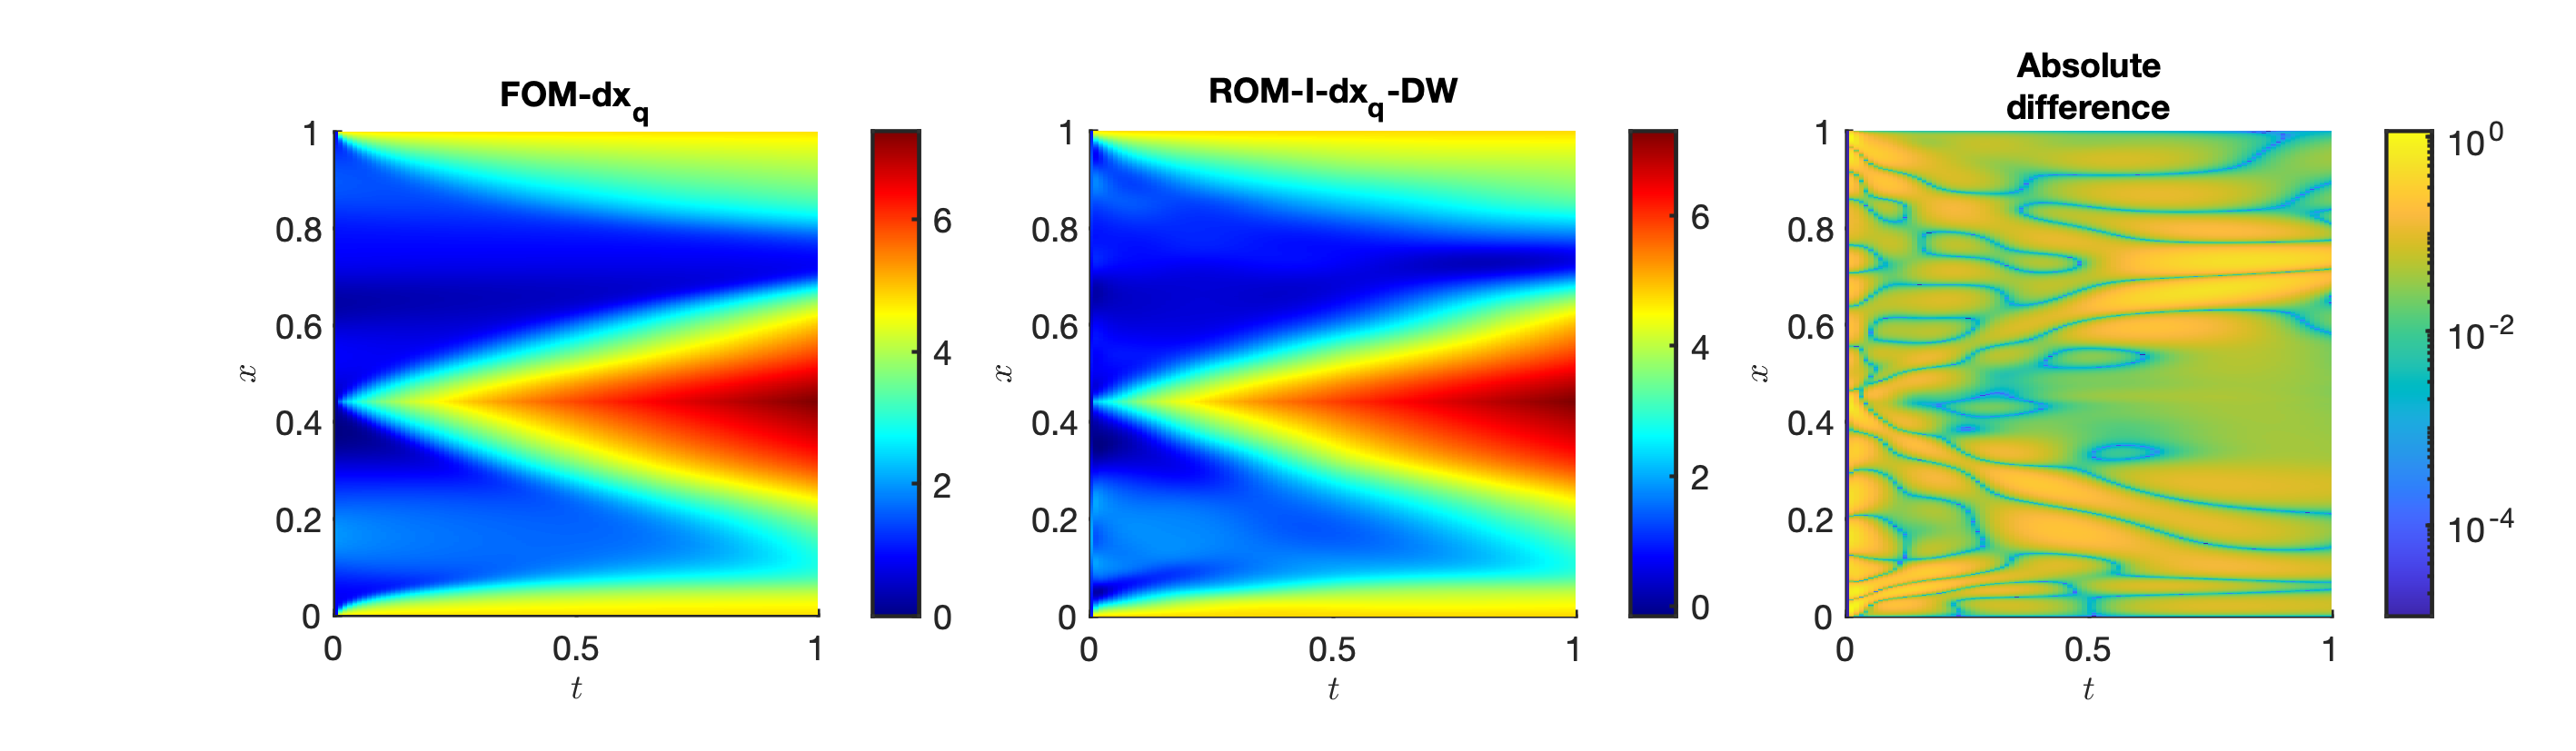
\includegraphics[width=\textwidth,trim={2.5cm 0 0 0},clip]{sci_report/images/ECMOR/14-Result-Q.png}
    }
    \caption{\todo{caption}~\cite{Elizarev2022}}\label{fig:q-domains}
\end{figure}

\begin{align}
    \deriv{u}{t} - \varkappa \left(\deriv[2]{u}{x} + \deriv[2]{u}{y} \right) = q \\
    \deriv{\check{y}}{y} = \gamma = \text{const}
\end{align}

\begin{equation}
    \deriv{u}{\check{t}} - \frac{\varkappa }{\alpha} \left(
        \beta^2 \deriv[2]{u}{\check{x}} + \gamma^2 \deriv[2]{u}{\check{y}}
        \right) = \frac{q}{\alpha}
\end{equation}

\begin{align}
    \matr{U}_{X} = \begin{bmatrix}
        \dots \\
        \matr{U}_{X_i}\\
         \dots
    \end{bmatrix}
    \in \mathbb{R}^{N_x \times N_y (N_{t}+1)} \\
    \matr{U}_{Y} = \begin{bmatrix}
        \dots \\
        \matr{U}_{Y_j}\\
         \dots
    \end{bmatrix}
    \in \mathbb{R}^{N_y \times N_x (N_{t}+1)} \\
    \matr{U}_{X_i} \rightarrow \widetilde{\Phi}_{X_i} \\
    \matr{U}_{Y_j} \rightarrow \widetilde{\Phi}_{Y_j}
\end{align}

\begin{align}
    \widetilde{\Phi}_{ij} \matr{R}_\text{qr}
    = \widetilde{\Phi}_{X_i} \otimes \widetilde{\Phi}_{Y_j} \\
\end{align}

\begin{align}
    d(x,t) : \left. u \right\vert_{x_{q2}}(x,t) = \left. u \right\vert_{x_{q1}}(d(x,t),t)
\end{align}
